
\subsection{简介}

\begin{enumerate}
\item Link/Cut Tree 是一种数据结构, 我们用它来解决 动态树问题
\item Link/Cut Tree 又称 Link-Cut Tree,简称 LCT, 但它不叫动态树,动态树是指一类问题。
\item Splay Tree 是 LCT 的基础, 但是 LCT ⽤的 Splay Tree 和普通的 Splay 在细节处不太一样。
\item 这是⼀个和 Splay ⼀样只需要写⼏ (yi) 个 (dui) 核心函数就能实现一切的数据结构。
\end{enumerate}

\subsection{问题引入}

\begin{itemize}
\item 维护一棵树, 支持如下操作。
\item 修改两点间路径权值。
\item 查询两点间路径权值和。
\item 修改某点子树权值。
\item 查询某点子树权值和。
  唔, 看上去是一道树剖模版题。
\end{itemize}

那么我们加两个操作

\begin{itemize}
\item 断开并连接⼀一些边, 保证仍是⼀一棵树。
\item 在线求出上⾯面的答案。
\end{itemize}

——动态树问题的解决方法:Link/Cut Tree!

\subsection{动态树问题}

\begin{itemize}
\item 维护一个 森林, 支持删除某条边, 加⼊某条边, 并保证加边, 删边之后仍是森林。我们要维护这个森林的一些信息。
\item 一般的操作有两点连通性, 两点路径权值和, 连接两点和切断某条边、修改信息等。
\end{itemize}

\hr

\subsubsection{从 LCT 的角度回顾一下树链剖分}

\begin{itemize}
\item 对整棵树按子树⼤小进⾏剖分, 并重新标号。
\item 我们发现重新标号之后, 在树上形成了一些以链为单位的连续区间, 并且可以用线段树进⾏区间操作。
\end{itemize}

\subsubsection{转向动态树问题}

\begin{itemize}
\item 我们发现我们刚刚讲的树剖是以子树⼤小作为划分条件。
\item 那我们能不能重定义一种剖分, 使它更适应我们的动态树问题呢?
\item 考虑动态树问题需要什么链。
\item 由于动态维护⼀个森林, 显然我们希望这个链是我们指定的链, 以便利⽤来求解。
\end{itemize}

\subsection{实链剖分}

\begin{itemize}
\item 对于⼀个点连向它所有⼉子的边 , 我们⾃己选择⼀条边进行剖分, 我们称被选择的边为实边, 其他边则为虚边。
\item 对于实边, 我们称它所连接的⼉子为实⼉子。
\item 对于⼀条由实边组成的链, 我们同样称之为实链。
\item 请记住我们选择实链剖分的最重要的原因: 它是我们选择的, 灵活且可变。
\item 正是它的这种灵活可变性, 我们采用 Splay Tree 来维护这些实链。
\end{itemize}

\subsection{LCT!}

\begin{itemize}
\item 我们可以简单的把 LCT 理解成用⼀些 Splay 来维护动态的树链剖分, 以期实现动态树上的区间操作。
\item 对于每条实链, 我们建⼀个 Splay 来维护整个链区间的信息。 
\item 接下来, 我们来学习 LCT 的具体结构。
\end{itemize}

\subsection{- 辅助树}

\begin{itemize}
\item 我们刚才在说的建树方法, 其实就是辅助树的建树方法, 我们先来 看⼀看辅助树的一些性质, 再通过一张图实际了解一下辅助树的具体结构。
\end{itemize}

\begin{enumerate}
\item 每⼀个 Splay 维护的是一条路径, 并且在原树中所有节点深度严格递增, 并且, 中序遍历这棵 Splay 得到的点序列列的点深度严格递增。
\item 每个节点包含且仅包含于一棵 Splay 中。
\item ⼀棵 Splay 的根节点的 Father 指向它在辅助树中的父亲结点。但是它父亲结点的 ch 并没有指向这个点的。即父亲不不⼀定认⼉子, ⽽⼉子能找到⽗亲。
\item 由于 LCT 的 Access 操作(后面会解释), 使得 3. 中的⽗亲不认⼉子对答案⽆任何影响, 同时, 也使一些叶⼦结点单独构成一棵 Splay 辅助树成为可能
\item 由于辅助树的以上性质, 我们维护任何操作都不不需要维护原树, 辅助树可以在任何情况下拿出一个唯一的原树, 我们只需要维护辅助树即可。(本句来源自 大爷 @PoPoQQQ 的 PPT)
\end{enumerate}

在本文里,你可以认为一些 Splay 构成了一个辅助树,每棵辅助树维护的是一棵树,一些辅助树构成了 LCT ,其维护的是整个森林。

\begin{itemize}
\item 现在我们有⼀棵原树, 如图。 
\item 加粗边是实边, 虚线边是虚边
\end{itemize}

\begin{figure}[h]
\centering
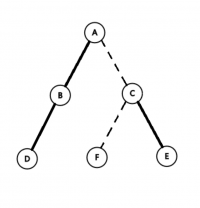
\includegraphics[width=0.5\textwidth]{images/lct9.png} 
\caption{lct9}
\end{figure}

\begin{itemize}
\item 由刚刚的定义, 辅助树的结构如下
\end{itemize}

\begin{figure}[h]
\centering
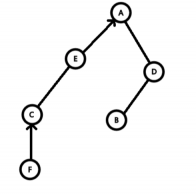
\includegraphics[width=0.5\textwidth]{images/lct10.png} 
\caption{lct10}
\end{figure}

\subsubsection{考虑原树和辅助树的结构关系}

\begin{itemize}
\item 原树中的实链 : 在辅助树中节点都在一棵 Splay 中
\item 原树中的虚链 : 在辅助树中, 子节点所在 Splay 的 Father 指向父节点, 但是父节点的两个儿子都不指向子节点。
\item 注意: 原树的根 ≠辅助树的根。
\item 原树的 Father 指向 ≠辅助树的 Father 指向。
\item 辅助树是可以在满足辅助树、Splay 的性质下任意换根的。
\item 虚实链变换可以轻松在辅助树上完成, 这也就是实现了动态维护树链剖分。
\end{itemize}

\subsubsection{接下来要用到的变量声明}

\begin{itemize}
\item \texttt{ch[N][2]} 左右⼉子 
\item \texttt{f[N]} ⽗亲指向
\item \texttt{sum[N]} 路径权值和 
\item \texttt{val[N]} 点权
\item \texttt{tag[N]} 翻转标记
\item \texttt{laz[N]} 权值标记 
\item Other\_Vars
\end{itemize}

\subsubsection{函数声明}

\paragraph{⼀般数据结构函数 (字面意思)}

\begin{enumerate}
\item PushUp(x)
\item PushDown(x)
\end{enumerate}

\paragraph{Splay 系函数 (不会多做解释)}

\begin{enumerate}
\item Get(x) 获取 x 是父亲的哪个⼉子。
\item Splay(x) 通过和 Rotate 操作联动实现把 x 旋转到 当前 Splay 的根。 
\item Rotate(x) 将 x 向上旋转一层的操作。
\end{enumerate}

\paragraph{新操作}

\begin{enumerate}
\item IsRoot(x) 判断当前节点是否是所在 Splay 的根
\item Access(x) 把从根到当前节点的所有点放在⼀条实链里, 使根到它成为一条实路径, 并且在同一棵 Splay 里里。
\item Update(x) 在 Access 操作之后, 递归的从上到下 Pushdown 更更新信 息。
\item MakeRoot(x) 使 x 点成为整个辅助树的根。
\item Link(x, y) 在 x, y 两点间连⼀一条边。
\item Cut(x, y) 把 x, y 两点间边删掉。
\item Find(x) 找到 x 所在的 Splay 的根节点编号。
\item Fix(x, v) 修改 x 的点权为 v。
\item Split(x, y) 提取出来 x, y 间的路路径, ⽅方便便做区间操作
\end{enumerate}

\subsubsection{宏定义}

\begin{itemize}
\item \texttt{#define ls ch[p][0]}
\item \texttt{#define rs ch[p][1]}
\end{itemize}

\subsection{函数讲解}

先从简单的来吧

\subsubsection{\texttt{PushUp()}}

\begin{cppcode}
inline void PushUp(int p) {
  __var1[p] =
      __var1[ls] "operator 1" __var1[rs] "operator 2" __var1[p] / __siz[p];
  siz[p] = siz[ls] + siz[rs];
}
\end{cppcode}

\subsubsection{\texttt{PushDown()}}

\begin{cppcode}
inline void PushDown(int p) {
  if (__tag1[p] != std_tag1) {
    // do ls & do rs
    __tag1[p] = std_tag1;
  }
}
\end{cppcode}

\subsubsection{\texttt{Splay() && Rotate()}}

有些不一样了哦

\begin{cppcode}
#define Get(x) (ch[f[x]][1] == x)
inline void Rotate(int x) {
  int y = f[x], z = f[y], k = Get(x);
  if (!isRoot(y)) ch[z][ch[z][1] == y] = x;
  // 上面这句一定要写在前面,普通的Splay是不用的,因为 isRoot  (后面会讲)
  ch[y][k] = ch[x][!k], f[ch[y][k]] = y;
  ch[x][!k] = y, f[y] = x, f[x] = z;
  PushUp(x), PushUp(y);
}
inline void Splay(int x) {
  Update(
      x);  // 马上就能看到啦。 在 Splay之前要把旋转会经过的路径上的点都PushDown
  for (int fa; fa = f[x], !isRoot(x); Rotate(x)) {
    if (!isRoot(fa)) Rotate(Get(fa) == Get(x) ? fa : x);
  }
}
\end{cppcode}

如果上面的几个函数你看不懂,请移步\href{/ds/splay/}{Splay} 

下面要开始 LCT 独有的函数了哦

\subsubsection{\texttt{isRoot()}}

\begin{cppcode}
// 在前面我们已经说过,LCT 具有 如果一个儿子不是实儿子,他的父亲找不到它的性质
// 所以当一个点既不是它父亲的左儿子,又不是它父亲的右儿子,它就是当前 Splay 的根
#define isRoot(x) (ch[f[x]][0] != x && ch[f[x]][1] != x)
\end{cppcode}

\subsubsection{Access() }

\begin{cppcode}
// Access 是 LCT
// 的核心操作,试想我们像求解一条路径,而这条路径恰好就是我们当前的一棵 Splay,
// 直接调用其信息即可 先来看一下代码,再结合图来看看过程
inline void Access(int x) {
  for (int p = 0; x; p = x, x = f[x]) {
    Splay(x), ch[x][1] = p, PushUp(x);
  }
}
\end{cppcode}

我们有这样一棵树,实线为实边,虚线为虚边 

\begin{figure}[h]
\centering
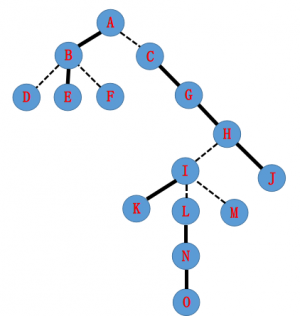
\includegraphics[width=0.5\textwidth]{images/lct1.png} 
\caption{pic1}
\end{figure}

\begin{itemize}
\item 它的辅助树可能长成这样 (构图方式不同可能 LCT 的结构也不同)
\item 每个绿框里是一棵 Splay。
\end{itemize}

\begin{figure}[h]
\centering
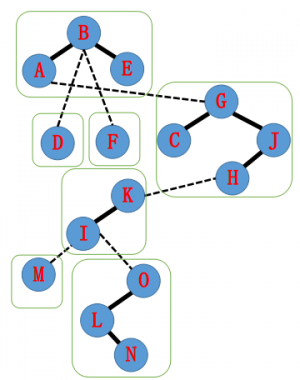
\includegraphics[width=0.5\textwidth]{images/lct2.png} 
\caption{pic2}
\end{figure}

\begin{itemize}
\item 现在我们要 Access(N), 把 A-N 的路径都变实, 拉成一棵 Splay
\end{itemize}

\begin{figure}[h]
\centering
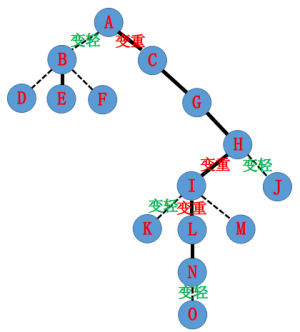
\includegraphics[width=0.5\textwidth]{images/lct3.png} 
\caption{pic3}
\end{figure}

\begin{itemize}
\item 实现的方法是从下到上逐步更新 Splay
\item 首先我们要把 N 旋至当前 Splay 的根。
\item 为了保证 AuxTree 的性质, 原来 N——O 的实边要更改为虚边。
\item 由于认父不认子的性质, 我们可以单方面的把 N 的儿子改为 Null。
\item 于是原来的 Aux 就从下图变成了下下图。
\end{itemize}

\begin{figure}[h]
\centering
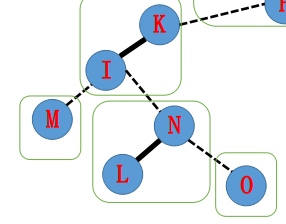
\includegraphics[width=0.5\textwidth]{images/lct4.png} 
\caption{pic4}
\end{figure}

\begin{figure}[h]
\centering
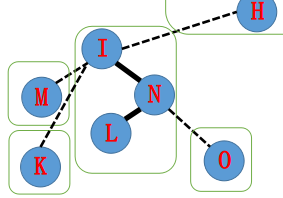
\includegraphics[width=0.5\textwidth]{images/lct5.png} 
\caption{pic}
\end{figure}

\begin{itemize}
\item 下一步, 我们把 N 指向的 Father-> I 也旋转到它 (I) 的 Splay 树根。
\item 原来的实边 I —— K 要去掉, 这时候我们把 I 的右儿子指向 N, 就得到了 I——L 这样一棵 Splay。
\end{itemize}

\begin{figure}[h]
\centering
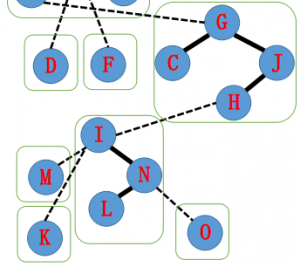
\includegraphics[width=0.5\textwidth]{images/lct8.png} 
\caption{pic}
\end{figure}

\begin{itemize}
\item 接下来, 按照刚刚的操作步骤, 由于 I 的 Father 指向 H, 我们把 H 旋转到他所在 Splay Tree 的根, 然后把 H 的 rs 设为 I。
\item 之后的树是这样的。
\end{itemize}

\begin{figure}[h]
\centering
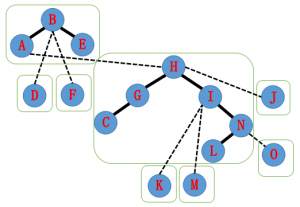
\includegraphics[width=0.5\textwidth]{images/lct6.png} 
\caption{pic}
\end{figure}

\begin{itemize}
\item 同理我们 Splay(A) , 并把 A 的右儿子指向 H。
\item 于是我们得到了这样一棵 AuxTree。并且发现 A——N 的整个路径已经在同一棵 Splay 中了。大功告成!
\end{itemize}

\begin{figure}[h]
\centering
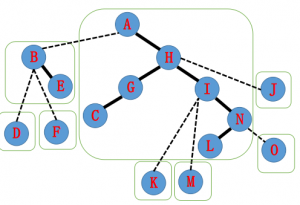
\includegraphics[width=0.5\textwidth]{images/lct7.png} 
\caption{pic}
\end{figure}

\begin{cppcode}
// 回顾一下代码
inline void Access(int x) {
  for (int p = 0; x; p = x, x = f[x]) {
    Splay(x), ch[x][1] = p, PushUp(x);
  }
}
\end{cppcode}

我们发现 Access() 其实很容易。只有如下四步操作:

\begin{enumerate}
\item 把当前节点转到根。
\item 把儿子换成之前的节点。
\item 更新当前点的信息。
\item 把当前点换成当前点的父亲, 继续操作。
\end{enumerate}

\subsubsection{\texttt{Update()}}

\begin{cppcode}
// 从上到下一层一层pushDown 即可
void Update(int p) {
  if (!isRoot(p)) Update(f[p]) pushDown(p);
}
\end{cppcode}

\subsubsection{\texttt{makeRoot()}}

\begin{itemize}
\item Make\_Root() 的重要性丝毫不亚于 Access() 。 我们在需要维护路径信息的时候, 一定会出现路径深度无法严格递增的情况, 根据 Aux 的性质, 这种路径是不能出现在一棵 Splay 中的。
\item 这时候我们需要用到 Make\_Root()。
\item Make\_Root() 。的作用是使指定的点成为原树的根, 考虑如何实现这种操作。
\item 我们发现 Access(x) 后,  x 在 Splay 中一定是深度最大的点 (从根到 x, 深度严格递增)。
\item 而变成根即是变成深度最小的点。我们 Splay(x) , 发现这时候 x 并没有右子树 (即所有点深度都比它浅)。那我们把 x 的左右儿子交换一下, 变成了 x 没有左子树, 在 Aux 意义上就是深度最小的点了, 即达到目的。
\item 所以我们交换左右儿子, 并给右儿子打一个翻转标记即可。(此时左儿子没有值)。
\end{itemize}

\begin{cppcode}
inline void makeRoot(int p) {
  Access(p), Splay(p);
  swap(ls, rs);
  tag[p] ^= 1;
}
\end{cppcode}

\subsubsection{\texttt{Link()}}

\begin{itemize}
\item Link 两个点其实很简单,  先 Make\_Root(x) , 然后把 x 的父亲指向 y 即可。显然, 这个操作肯定不能发生在同一棵树内 OTZ。记得先判一下。
\end{itemize}

\begin{cppcode}
inline void Link(int x, int p) {
  makeRoot(x);
  f[x] = p;
}
\end{cppcode}

\subsubsection{\texttt{Split()}}

\begin{itemize}
\item Split 操作意义很简单, 就是拿出一棵 Splay , 维护的是 x 到 y 的路径。
\item 先 MakeRoot(x) , 然后 Access(y) 。如果要 y 做根, 再 Splay(y) 。
\item 就这三句话, 没写代码, 需要的时候可以直接打这三个就好辣!
\item 另外 Split 这三个操作直接可以把需要的路径拿出到 y 的子树上, 那不是随便干嘛咯。
\end{itemize}

\subsubsection{\texttt{Cut()}}

\begin{itemize}
\item Cut 有两种情况, 保证合法和不一定保证合法。(废话)
\item 如果保证合法, 直接 split(x, y) , 这时候 y 是根, x 一定是它的儿子, 双向断开即可 , 就像这样:
\end{itemize}

\begin{cppcode}
inline void Cut(int x, int p) {
  makeRoot(x), Access(p), Splay(p), ls = f[x] = 0;
}
\end{cppcode}

如果是不保证合法, 我们需要判断一下是否有, 我选择使用 Map 存一下, 但是这里有一个利用性质的方法:

想要删边, 必须要满足如下三个条件:

\begin{enumerate}
\item x, y 连通。
\item x, y 的路径上没有其他的链。
\item x 没有右儿子。
\item 总结一下, 上面三句话的意思就一个:x, y 有边。
\end{enumerate}

具体实现就留作一个思考题给大家。判断连通需要用到后面的 Find , 其他两点稍作思考分析一下结构就知道该怎么判断了。

\subsubsection{\texttt{Find()}}

\begin{itemize}
\item Find() 其实就是找到当前辅助树的根。在 Access(p) 后, 再 splay(p)。这样根就是树里最小的那个, 一直往 ls 走, 沿途 PushDown 即可。
\item 一直走到没有 ls, 非常简单。
\end{itemize}

\begin{cppcode}
inline int Find(int p) {
  Access(p), Splay(p);
  while (ls) pushDown(p), p = ls;
  return p;
}
\end{cppcode}

\subsubsection{一些提醒}

\begin{itemize}
\item 干点啥一定要想一想需不需要 PushUp 或者 PushDown, LCT 由于特别灵活的原因, 少 Pushdown 或者 Pushup 一次就可能把修改改到不该改的点上!
\item 它的 rotate 和 splay 的不太一样, if(z) 一定要放在前面。
\item 它的 splay 就是旋转到根, 没有旋转到谁儿子的操作, 因为不需要。
\end{itemize}

\subsection{一些题}

\begin{itemize}
\item BZOJ\_2049 
\item BZOJ\_3282
\item BZOJ\_2002
\item BZOJ\_2631
\end{itemize}
